\documentclass[twocolumn,a4j]{jsarticle}
\setlength{\topmargin}{-20.4cm}
\setlength{\oddsidemargin}{-10.4mm}
\setlength{\evensidemargin}{-10.4mm}
\setlength{\textwidth}{18cm}
\setlength{\textheight}{26cm}
\renewcommand{\figurename}{fig.}
\renewcommand{\tablename}{table }

\usepackage[top=15truemm,bottom=25truemm,left=20truemm,right=20truemm]{geometry}
\usepackage[latin1]{inputenc}
\usepackage{amsmath}
\usepackage{amsfonts}
\usepackage{amssymb}
\usepackage{listings}
\usepackage{listings,jvlisting}
\usepackage{geometry}
\usepackage{enumerate}
\usepackage[dvipdfmx]{graphicx}
\usepackage[dvipdfmx]{hyperref}
\usepackage{comment}

\makeatletter
\def\@maketitle
{
\begin{center}
{\LARGE \@title \par}
\end{center}
\begin{flushright}
{\large 報告書NO.03\quad\@date\quad\@author}
\end{flushright}
\par\vskip 1.5em
}
\makeatother

\author{来代 勝胤}
\title{令和3年度 6月 報告書}
\date{2021/7/7}

\begin{document}
\maketitle
\section*{報告内容}
\begin{itemize}
    \item 進捗概要
    \item 揚抗力測定の事前実験
          % \item Arduinoによる温湿度測定
    \item 7月の予定
\end{itemize}
\section{進捗概要}
今月は、揚抗力測定の事前実験を行った。
具体的に行った実験の内容は以下の通りである。
\begin{enumerate}[(1)]
    \item ロードセルの校正実験
    \item タイヤモデルとロードセルの校正実験
\end{enumerate}
\section{揚抗力測定の事前実験}
\subsection{実験の目的と方法}
作用力測定の実験を行うにあたり、タイヤモデルの上方に設置されているひずみゲージの出力電圧と
実際に加わっている荷重を関係付ける必要がある。
そこで、ロードセルを用いた校正実験を行うことによりそれらを行った。
以下の(1)から(3)の過程から作用力の測定を行うことができると考えている。
\begin{enumerate}[(1)]
    \item ひずみゲージとロードセルの出力電圧の関係を調べる
    \item ひずみゲージの出力電圧と荷重の関係を調べる
    \item 導出した関係をもとにひずみゲージの出力電圧から作用力を求める
\end{enumerate}
現在、$\left(1\right)$、$\left(2\right)$の実験結果の取得まで終了している。
しかし結果の分析等は十分にできていないため、簡易的に分析を行った$\left(2\right)$の結果を示す。\\
\subsection{ロードセルの校正実験}
ロードセルにおける出力電圧と荷重の関係を調べるために、
垂直に設置したロードセルの先にナットを吊るし、その電圧との関係を見ることで荷重と電圧を関係を示すこととした。
右上に実験の概略図を示す。
\begin{figure}[htbp]
    \begin{center}
        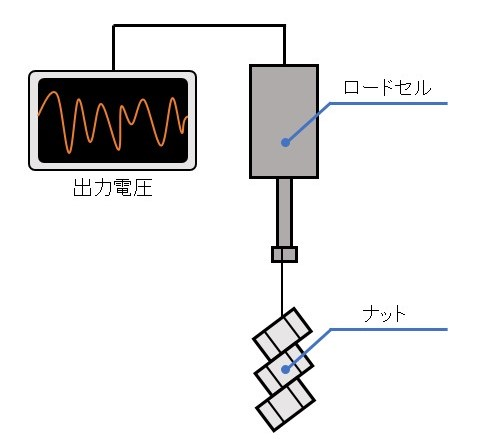
\includegraphics[width=70mm]{images/schematic.jpg}
        \caption{shematic}
        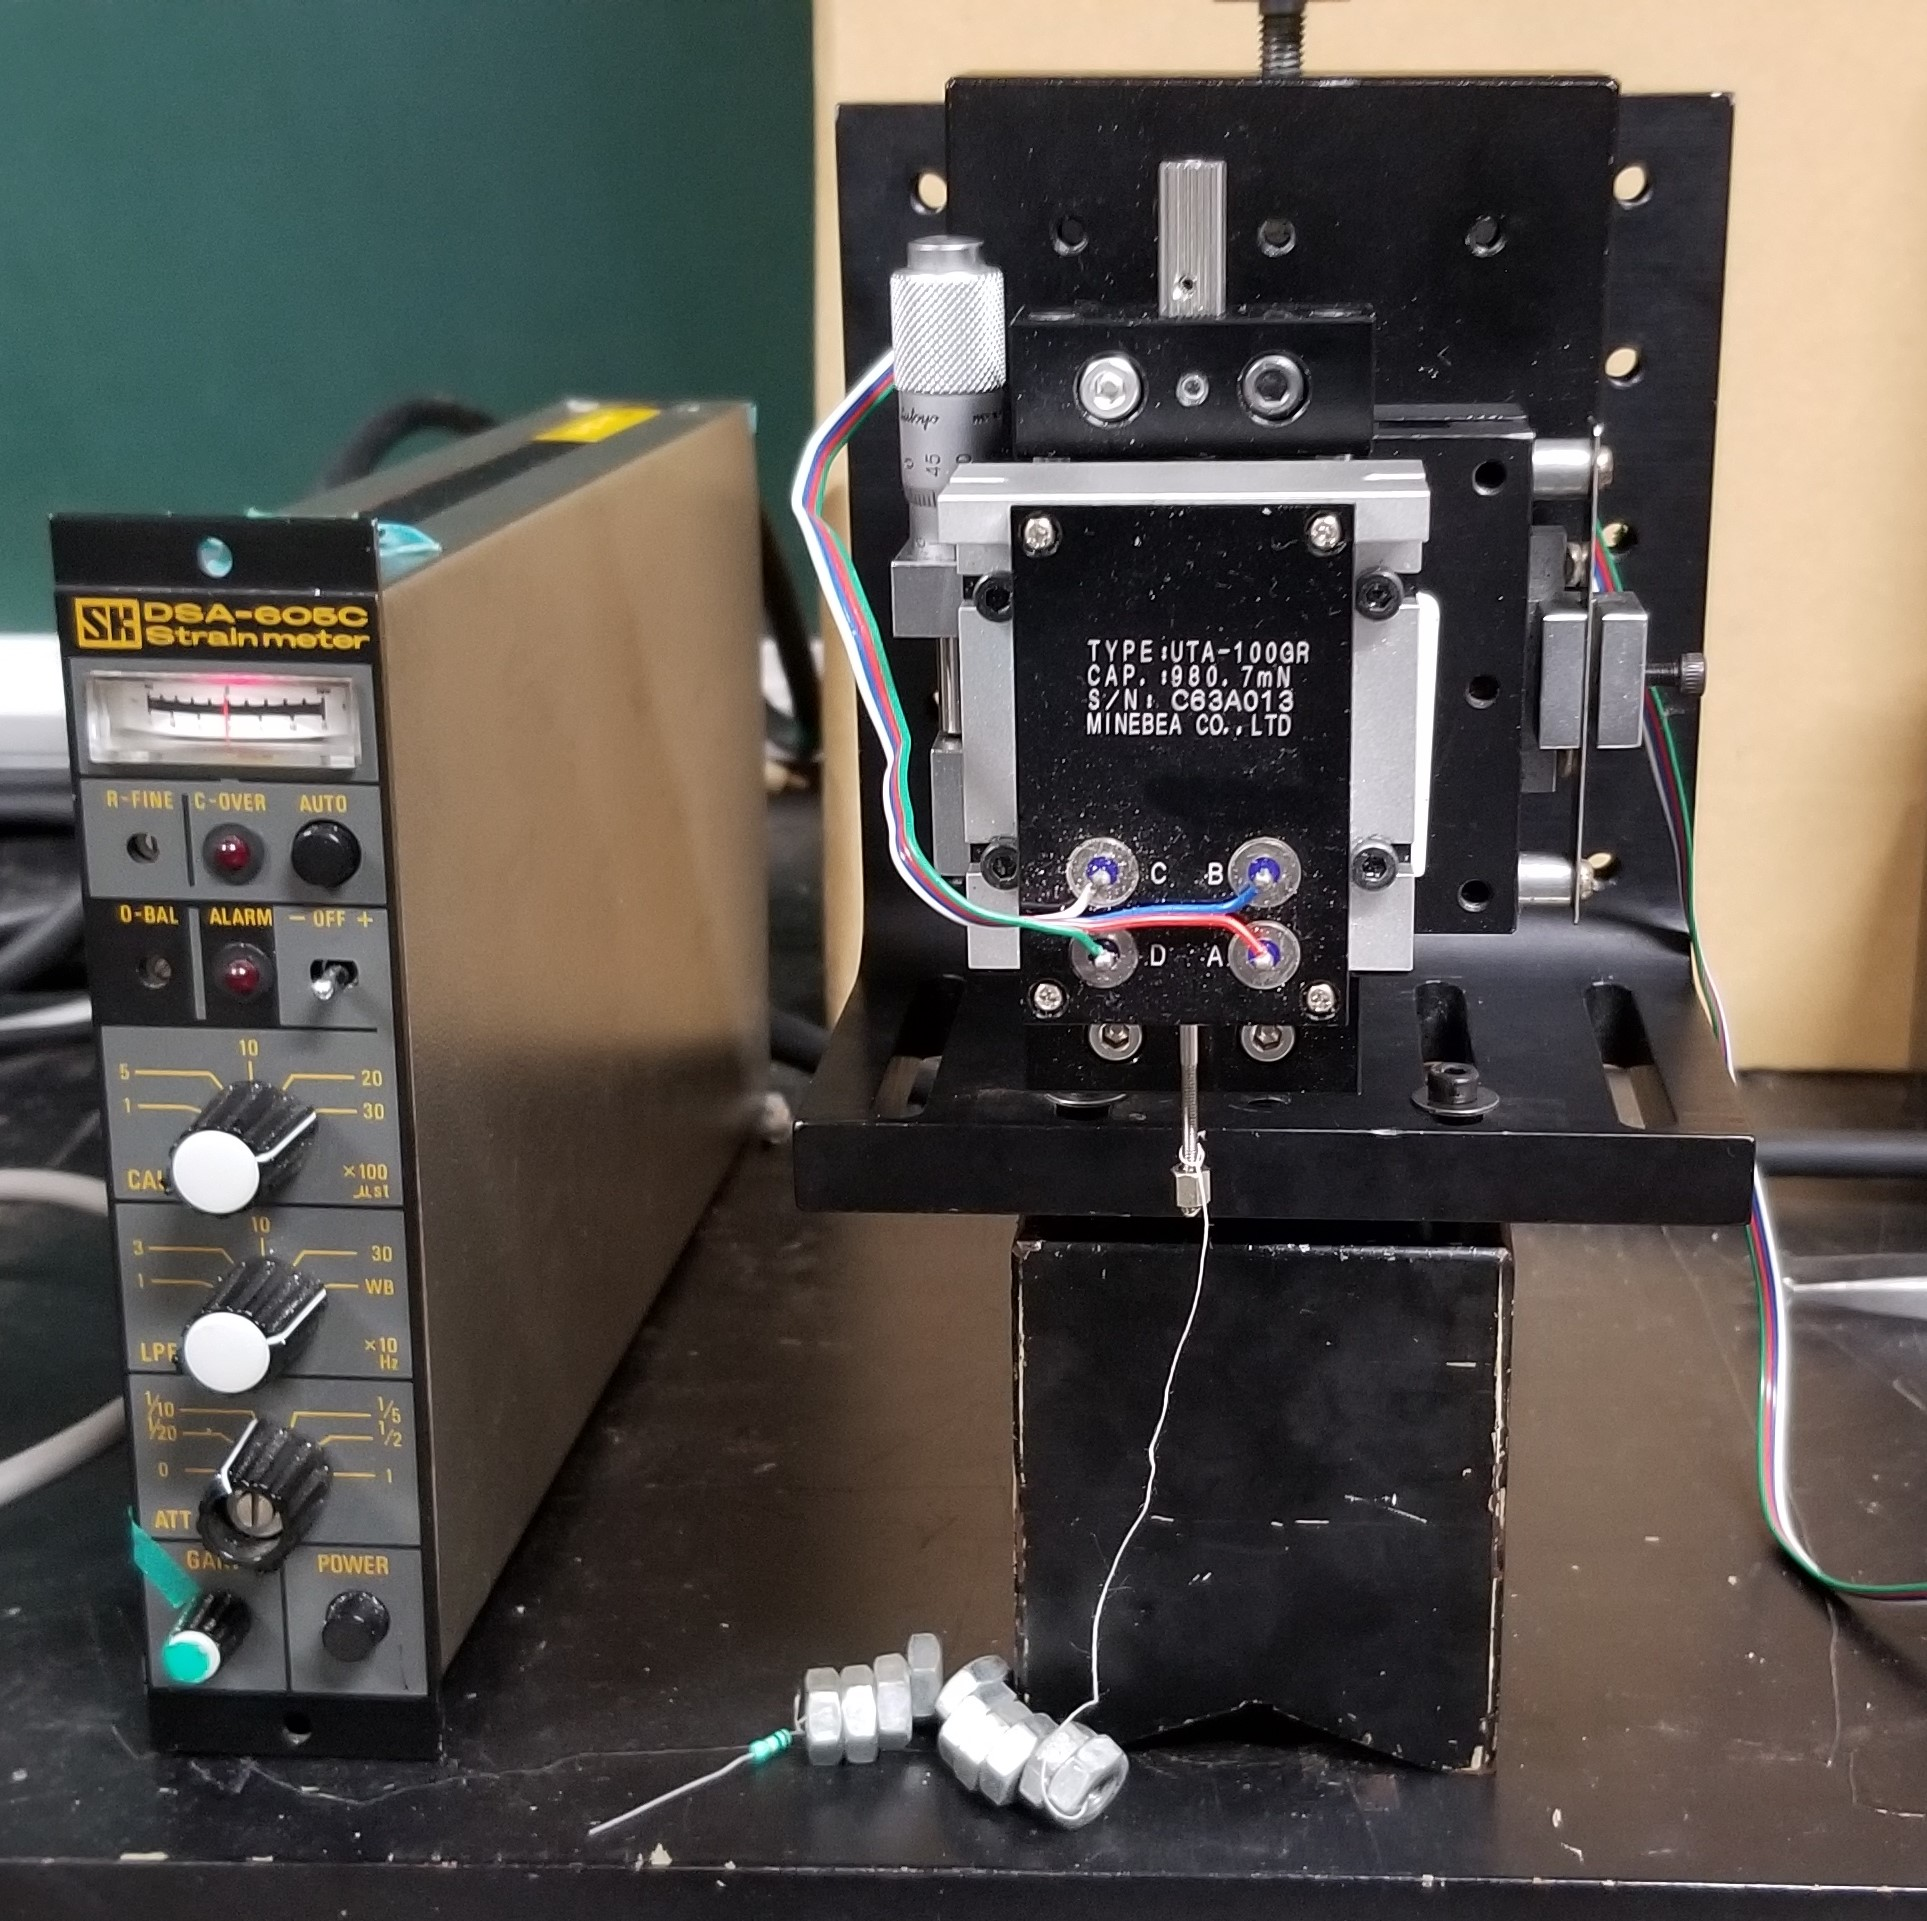
\includegraphics[width=70mm]{images/loadcell.jpg}
        \caption{experimental device}
    \end{center}
\end{figure}
\subsubsection{実験方法}
\begin{enumerate}[(1)]
    \item ロードセルを垂直に設置する
    \item ナット$\left(3.5 \mathrm{\left[g/個\right]}\right)$を1つずつ吊るしていき、その電圧を記録する。
          10個まで吊るし終わったら1つずつ取り外しその電圧を記録する。
    \item 以上を2回繰り返す。
\end{enumerate}
\subsubsection{実験結果}
また、簡易的ではあるが実験結果のグラフを以下に示す。
以下のグラフはexcelで作成し、破線は最小二乗法に基づいて作成された近似直線を示している。
また、各値は実験2セット分(各荷重につき4つの電圧の値)を平均したものを用いている。
\begin{figure}[htbp]
    \begin{center}
        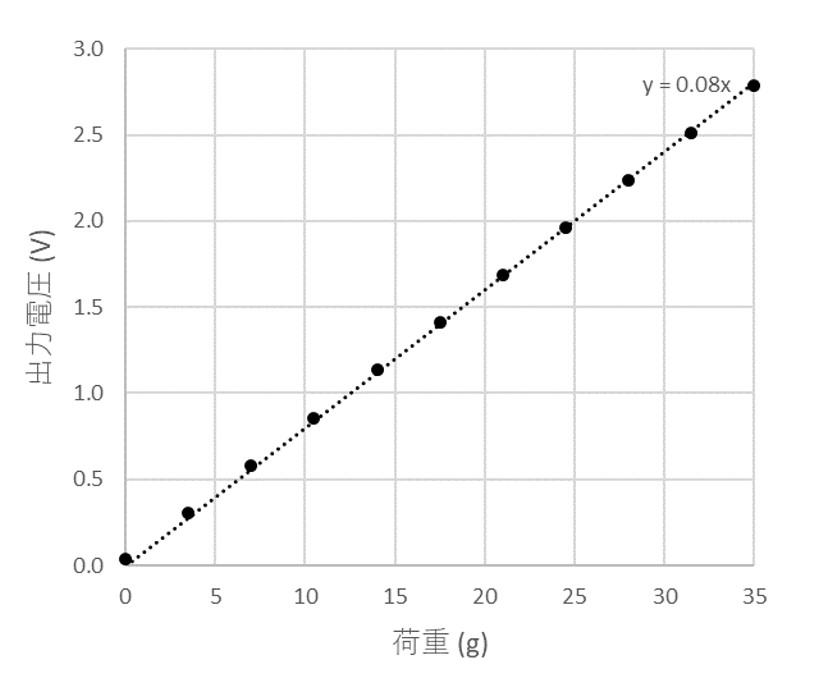
\includegraphics[width=60mm]{images/result.jpg}
        \caption{result}
    \end{center}
\end{figure}
\newpage
結果をみると、荷重と出力電圧との間に非常にきれいな比例関係があることがわかった。
しかしながら、実際にロードセルを用いてタイヤモデルに荷重をかける際には、
\begin{enumerate}[(1)]
    \item 荷重が圧縮方向に加わる
    \item ロードセルを水平方向に設置して使用する
\end{enumerate}
といった、校正実験とは異なる条件で使用されることもあるが、
今回はその影響の確認を行っていない。今後考慮が必要になる可能性がある要素のうちの1つであると考えられる。\\
\subsection{タイヤモデルとロードセルの校正実験}
タイヤモデルにロードセルを押し付けて荷重をかけ、
タイヤモデルに取り付けられたひずみゲージの出力電圧とロードセルの出力電圧を記録し、
2.2のロードセルの校正実験結果との関係を調べることが目的である。
実験は完了しているが、結果の分析を行うことができていないため入試後に行う予定である。
\begin{comment}
\newpage
\section{Arduinoを用いた温湿度計の製作}
Aruduino講習会が実施されていたため、その応用として温湿度計の製作した。
温湿度計については、\href{https://prod.kyohritsu.com/KP-AM2320.html}{KP-AM2320}を用いた。
\begin{figure}[htbp]
    \begin{center}
        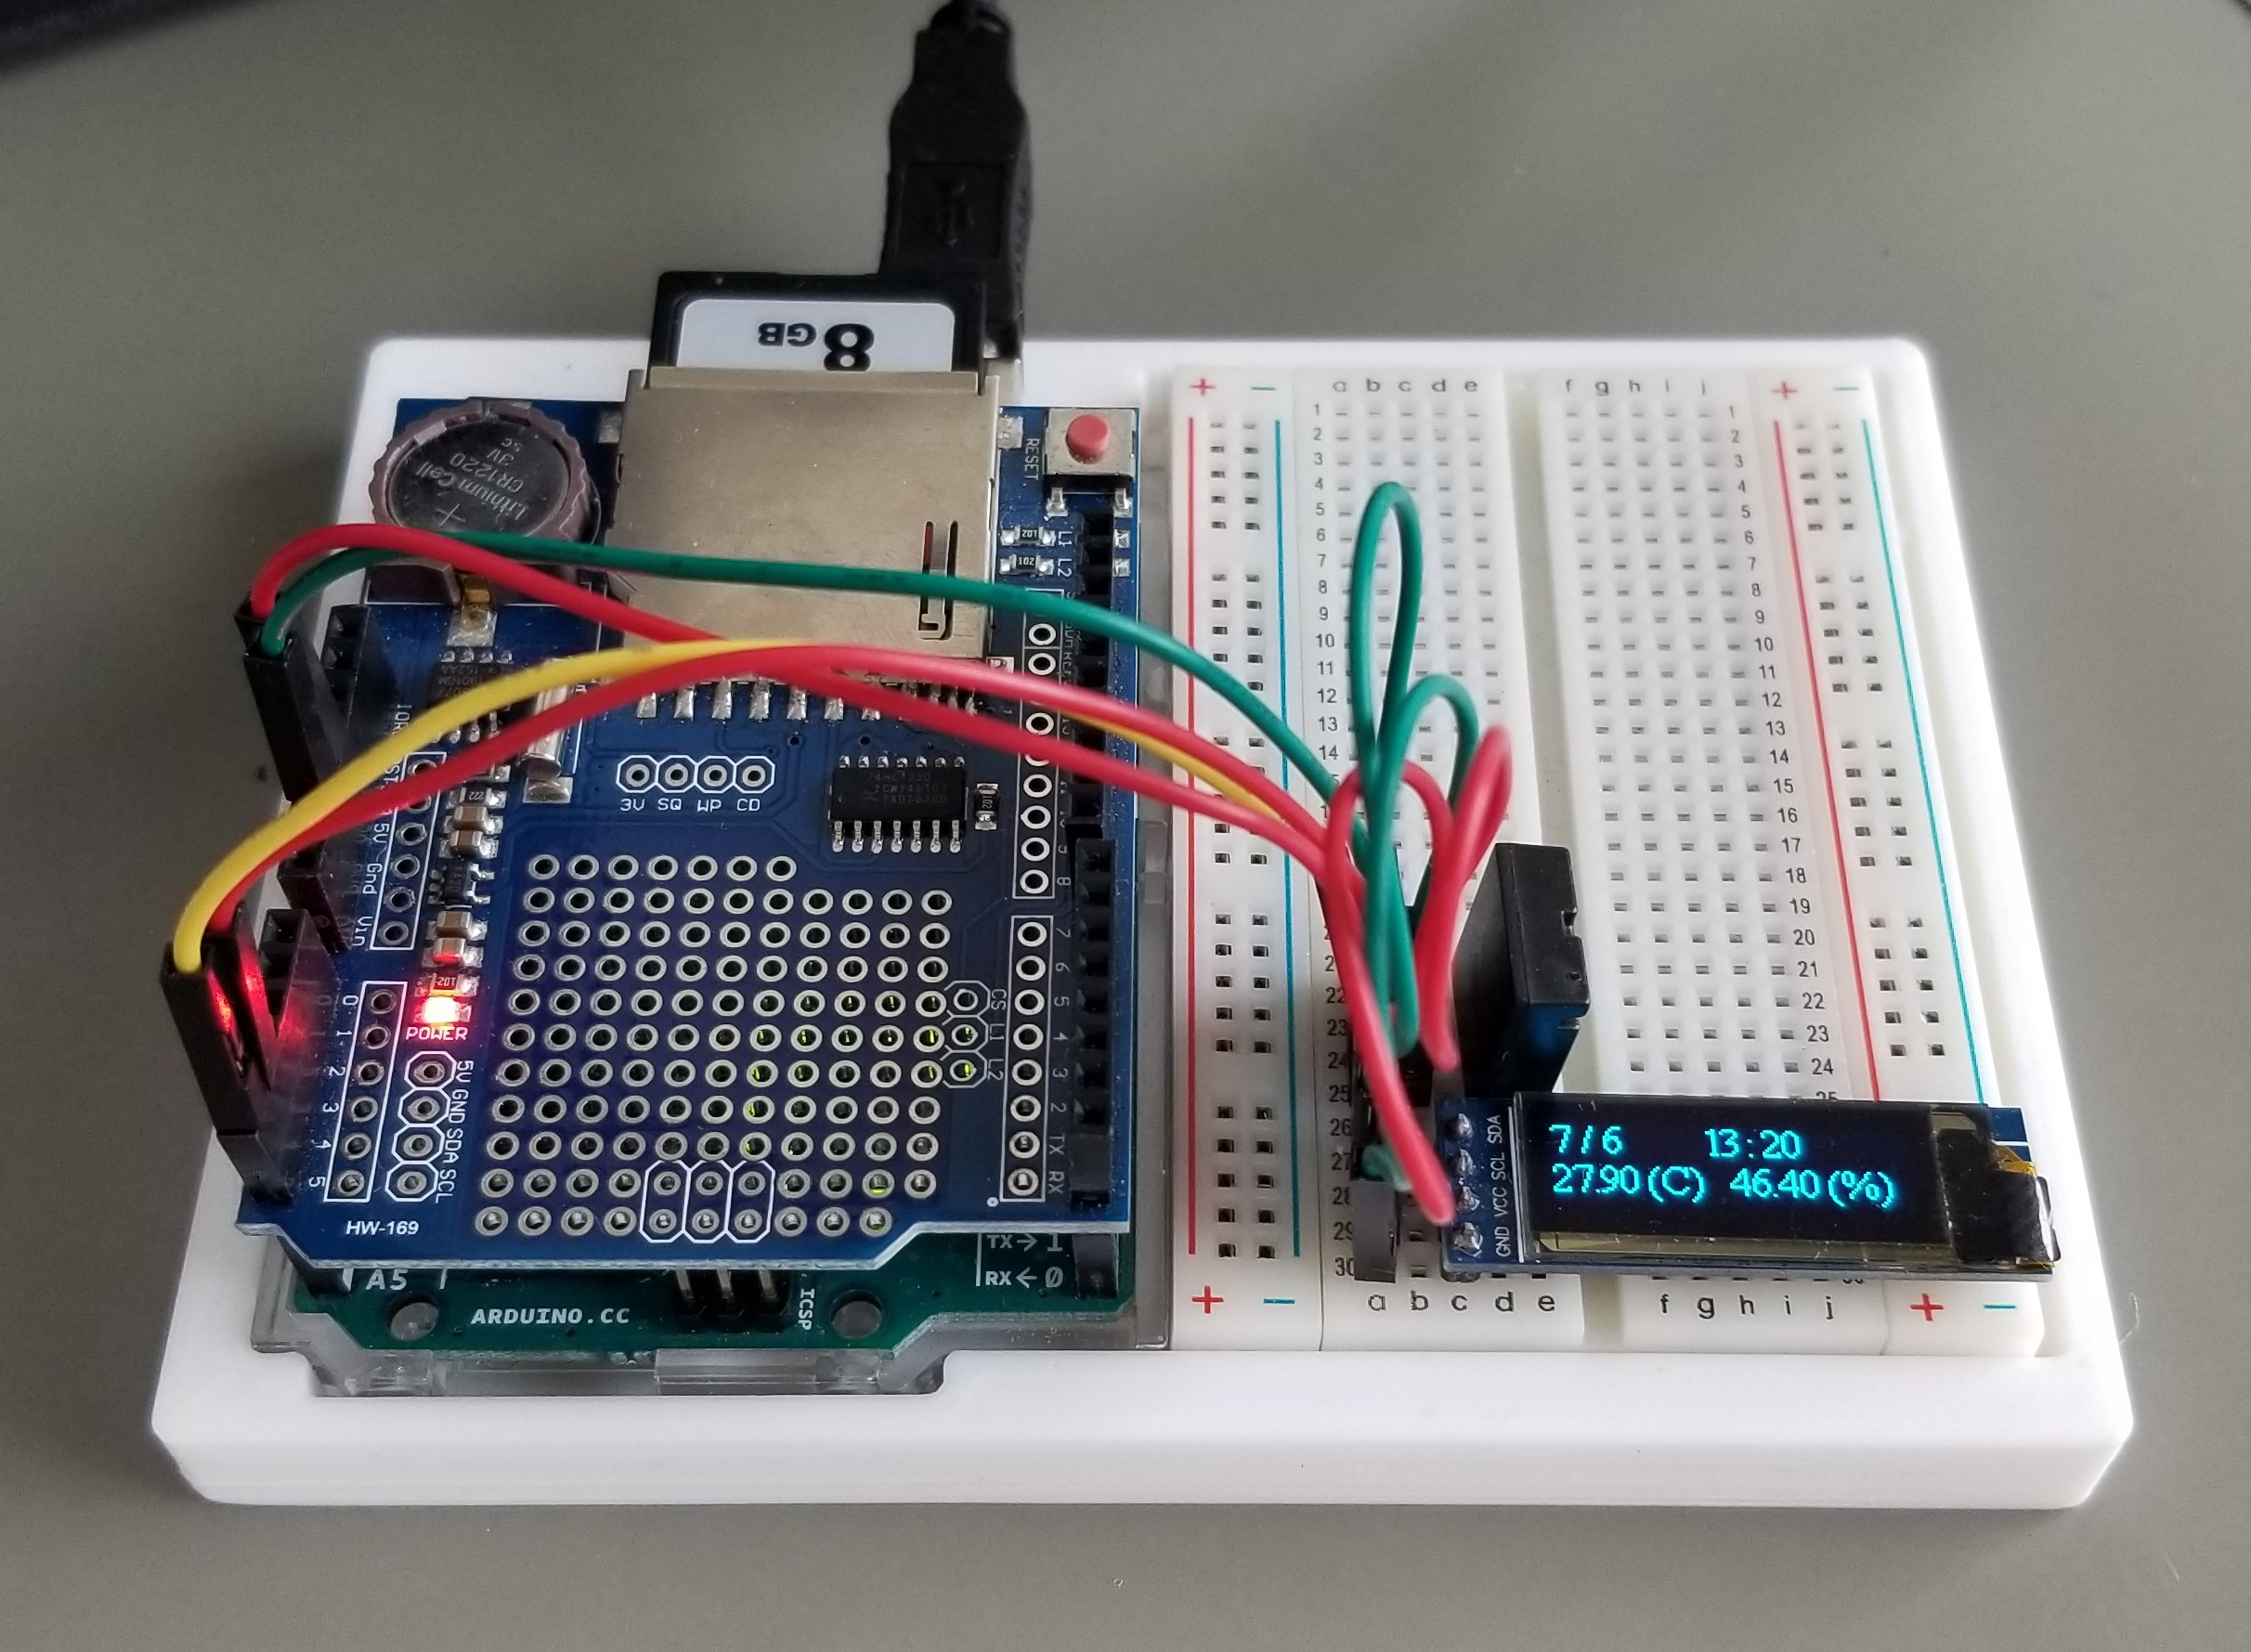
\includegraphics[width=60mm]{images/arduino.jpg}
        \caption{thermo-hygrometer}
    \end{center}
\end{figure}
温湿度センサから出力下データを画像手前の液晶モニタに表示し、
画像左上に挿入されているSDカードに1分ごとに記録できるようにしている。
\end{comment}
\section{7月の予定}
7月は、引越しの関係もあり、回流水槽を用いた実験ができなくなってしまうため、
タイヤの作用力測定を複数のモデルで行う必要がある。また、大学院入試が近づいてきたため
入試に向けた勉強を優先して行う。
\end{document}